\begin{frame}
\frametitle{Conditions and data}

\begin{table}[h!]
\caption{Conditions and data for run \runNumber}
\begin{center}
\begin{tabular}{|c|c|}
\hline
Conditions & Data \\
\hline
run number & \runNumber \\
file range & (0,8798) \\
date & <<date>> \\
lab temperature: & <<labTempC>> $\deg$ \\
Total number of S2s  &  <<totalNumS2>> \\
Total number of events & <<totalNumEvt>> \\
\hline
\end{tabular}
\end{center}
\label{r\runNumber.data}
\end{table}%
\end{frame}

\begin{frame}
\begin{figure}
  \begin{center}
      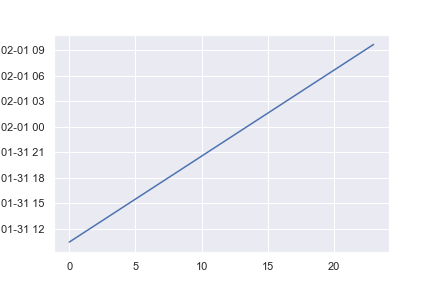
\includegraphics[width=0.45\textwidth]{img/r\runNumber x2rg_local_190819/runTime.png}
      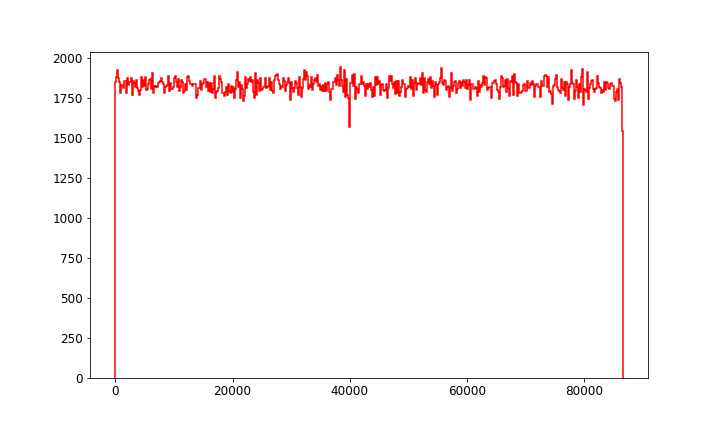
\includegraphics[width=0.45\textwidth]{img/r\runNumber x2rg_local_190819/runEvt.png}
    \caption{Run data.}
  \end{center}
\end{figure}
\end{frame}

\begin{frame}
\frametitle{S1 \& S2}

\begin{table}[h!]
\caption{S1 \& S2 for run \runNumber}
\begin{center}
\begin{tabular}{|c|c|}
\hline
Conditions & Data \\
\hline
fraction of S1s & <<fracS1>> \\
fraction of S2s (1 S1) & <<fracS2>> \\
fraction 1 S2 \& 1 S1 & <<fracS1S2>> \\
\hline
\end{tabular}
\end{center}
\label{r\runNumber.data}
\end{table}%

\begin{table}[h!]
\caption{S1 \& S2 selection for run \runNumber}
\begin{center}
\begin{tabular}{|c|c|}
\hline
Variables & Data \\
\hline
$s_1$~energy & <<s1Min>> pes to <<s1Max>> pes \\
$s_2$~energy (PMTs) & <<s2MinPMT>> pes to <<s2MaxPMT>> pes \\
$s_2$~charge (SiPMs) & <<s2MinQ>> pes to <<s2MaxQ>> pes \\
$s_2$~width & <<widthMin>> $\mu s$ to <<widthMax>> $\mu s$ \\
$n_{sipm}$~min & <<numSipmMin>>\\
\hline
\end{tabular}
\end{center}
\label{r\runNumber.sel}
\end{table}%
\end{frame}


\begin{frame}
\begin{figure}
  \begin{center}
      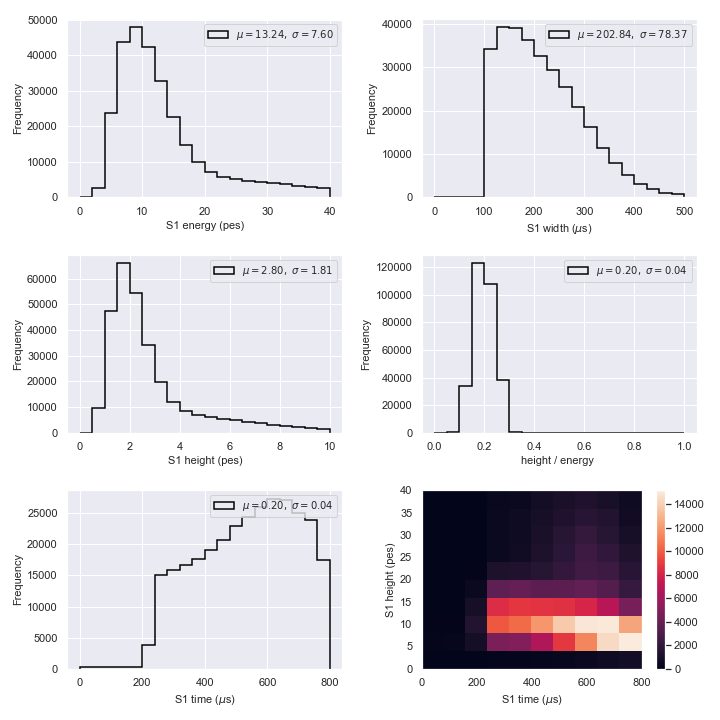
\includegraphics[width=0.6\textwidth]{img/r\runNumber x2rg_local_190819/s1.png}
    \caption{S1 distributions.}
  \end{center}
\end{figure}
\end{frame}

\begin{frame}
\begin{figure}
  \begin{center}
      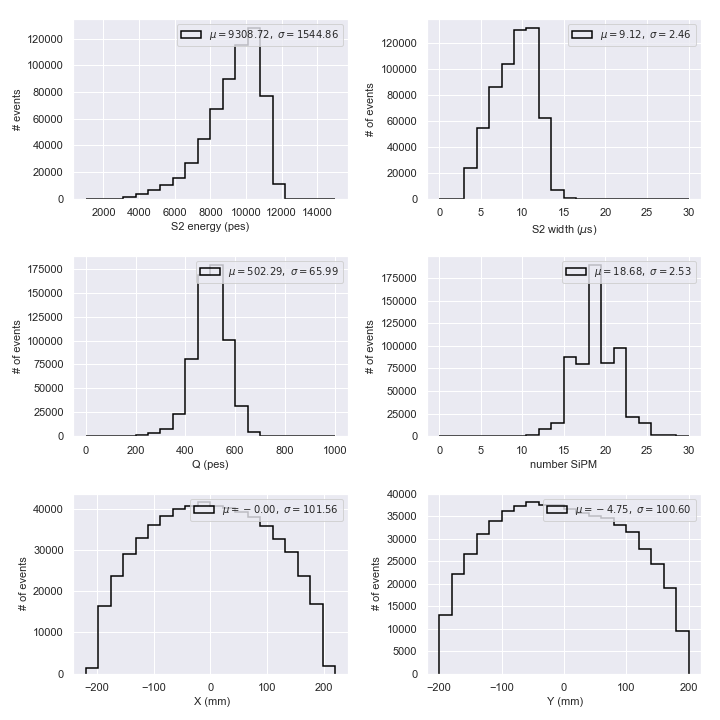
\includegraphics[width=0.6\textwidth]{img/r\runNumber x2rg_local_190819/s2.png}
    \caption{S2 distributions.}
  \end{center}
\end{figure}
\end{frame}

\begin{frame}
\frametitle{Control distributions}
\begin{figure}
  \begin{center}
      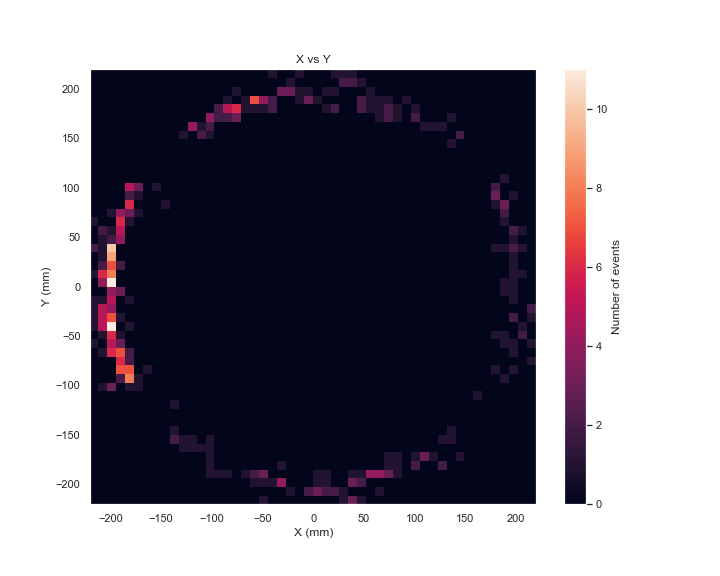
\includegraphics[width=0.6\textwidth]{img/r\runNumber x2rg_local_190819/xy.png}
    \caption{XY distribution.}
  \end{center}
\end{figure}
\end{frame}

\begin{frame}
\begin{figure}
  \begin{center}
      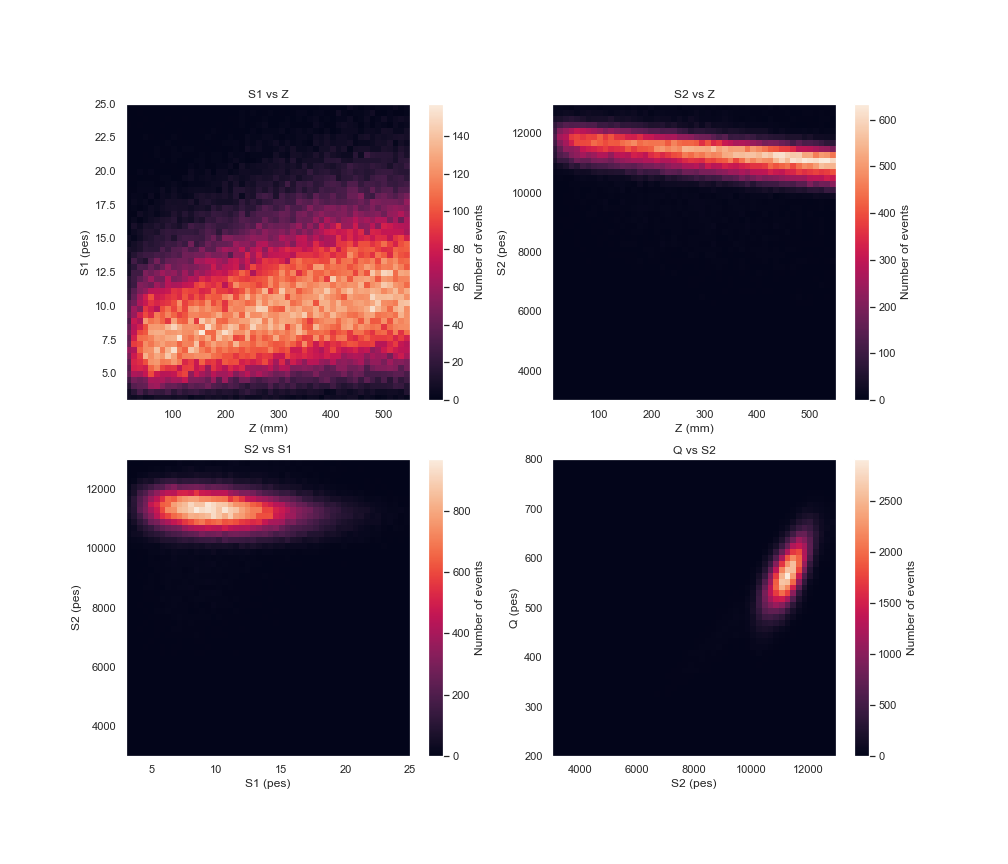
\includegraphics[width=0.7\textwidth]{img/r\runNumber x2rg_local_190819/s1s2q.png}
    \caption{S1, S2 \& Q distributions.}
  \end{center}
\end{figure}
\end{frame}

\begin{frame}
\frametitle{Lifetime distributions}
\begin{figure}
  \begin{center}
      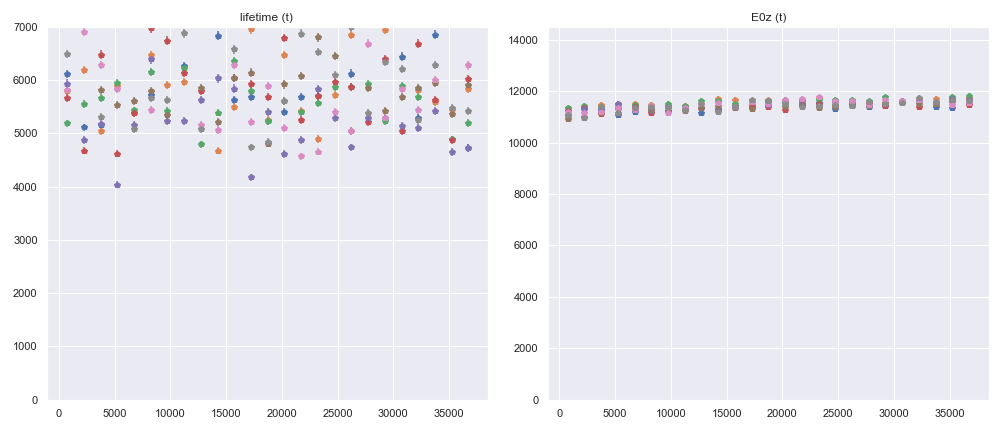
\includegraphics[width=0.4\textwidth]{img/r\runNumber x2rg_local_190819/R_phi_lt1.png}
      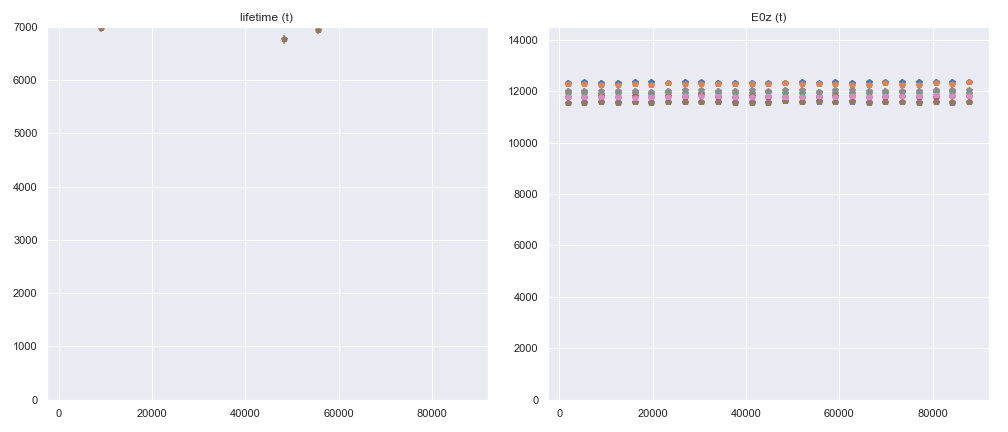
\includegraphics[width=0.4\textwidth]{img/r\runNumber x2rg_local_190819/R_phi_lt2.png} \\
      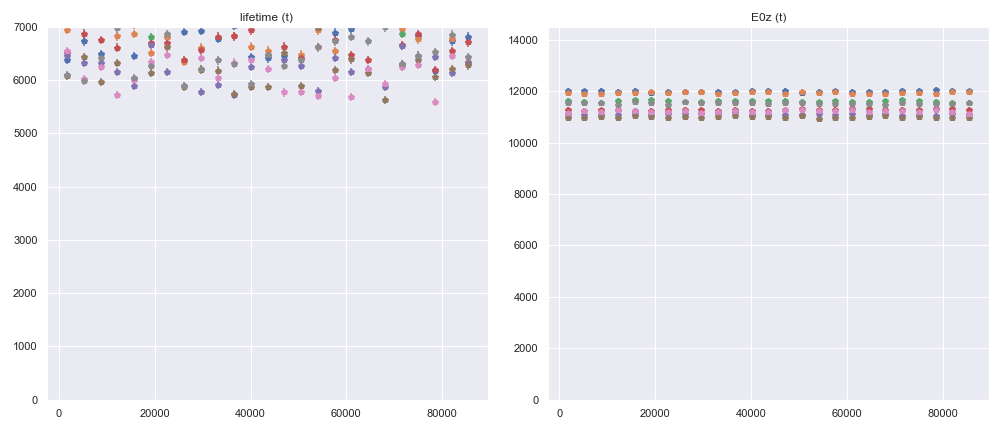
\includegraphics[width=0.4\textwidth]{img/r\runNumber x2rg_local_190819/R_phi_lt3.png}
      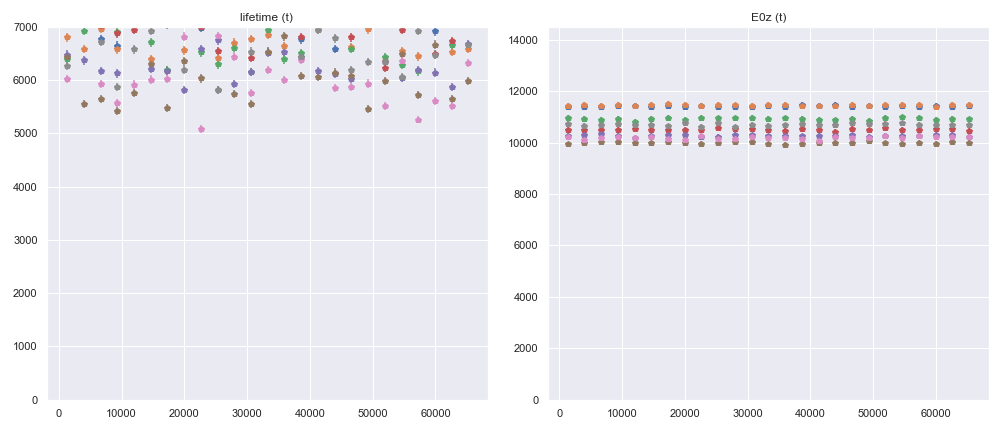
\includegraphics[width=0.4\textwidth]{img/r\runNumber x2rg_local_190819/R_phi_lt4.png}\\
      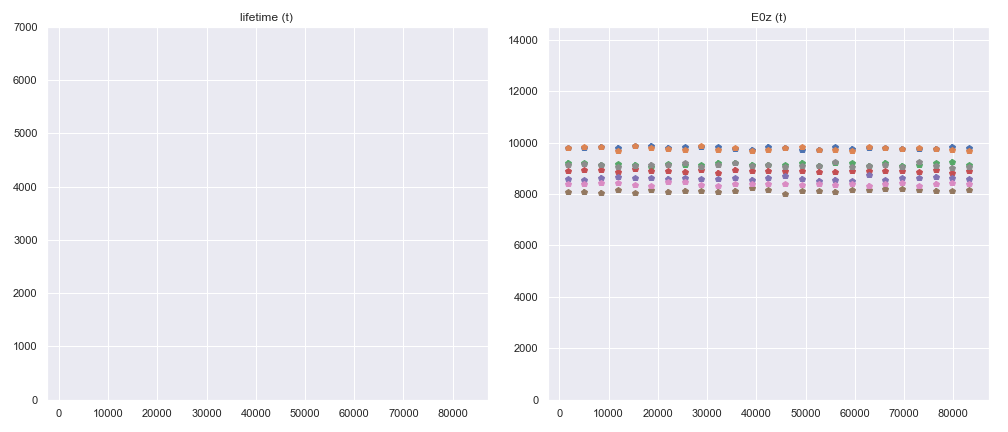
\includegraphics[width=0.4\textwidth]{img/r\runNumber x2rg_local_190819/R_phi_lt5.png}
    \caption{Distributions of lifetime and $E_0$~for 5 radial sectors (40, 80, 120, 160, 200).}
  \end{center}
\end{figure}
\end{frame}

\begin{frame}
\frametitle{Lifetime maps}
\begin{figure}
  \begin{center}
      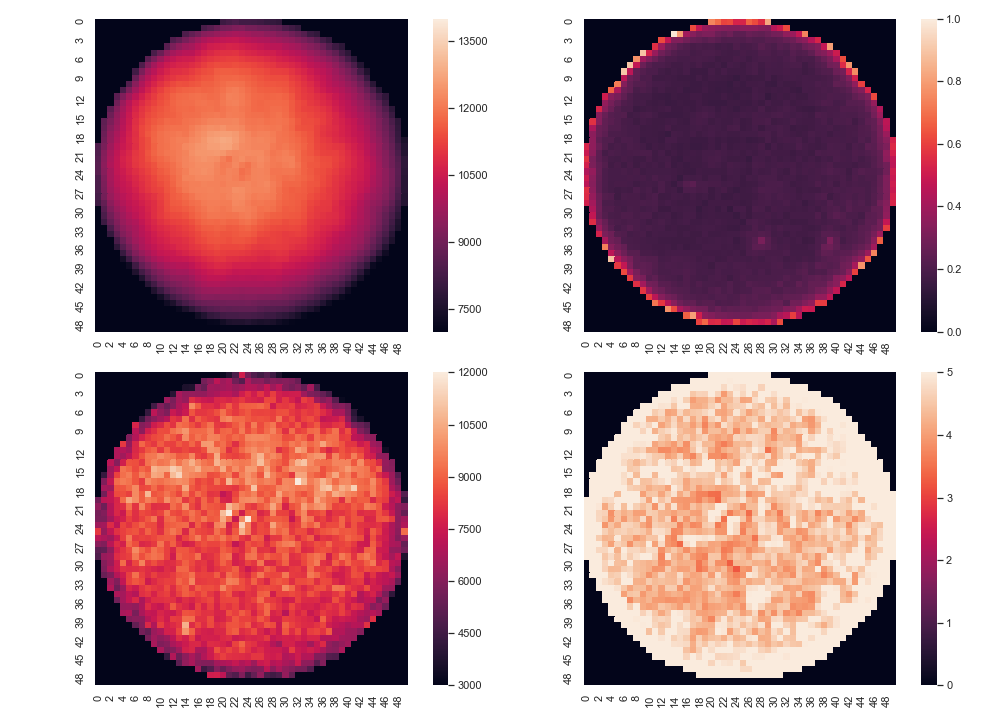
\includegraphics[width=0.7\textwidth]{img/r\runNumber x2rg_local_190819/maps.png}
    \caption{Lifetime and geometrical map.}
  \end{center}
\end{figure}
\end{frame}

\begin{frame}
\frametitle{Lifetime maps}
\begin{figure}
  \begin{center}
      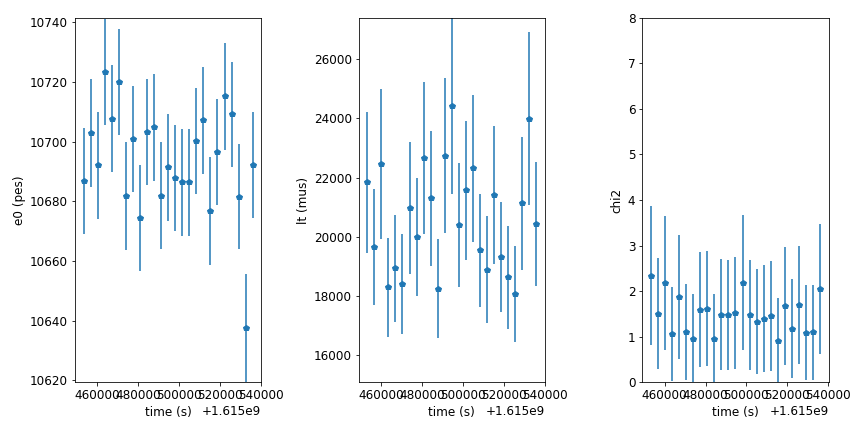
\includegraphics[width=0.7\textwidth]{img/r\runNumber x2rg_local_190819/AverageLT.png}
    \caption{Average lifetime.}
  \end{center}
\end{figure}
\end{frame}

\begin{frame}
\frametitle{Lifetime and geometry correction}
\begin{figure}
  \begin{center}
      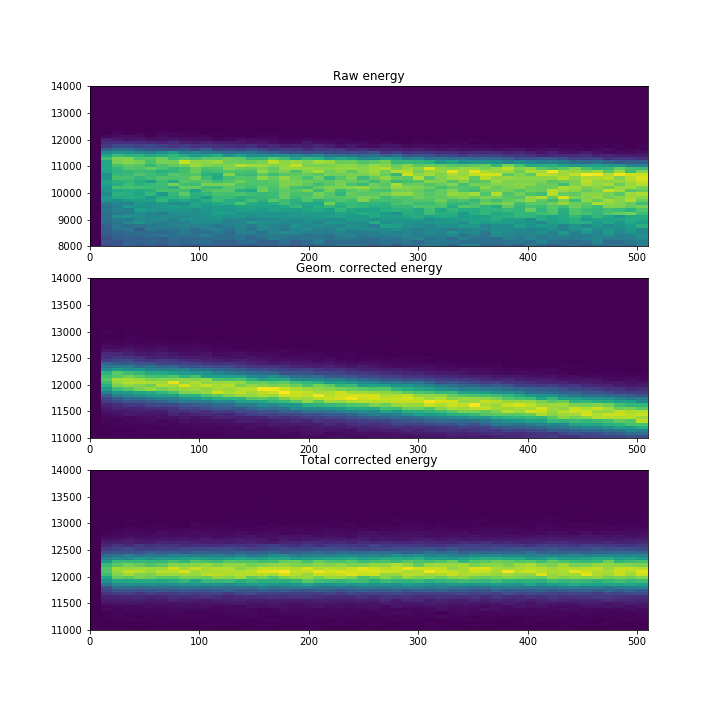
\includegraphics[width=0.7\textwidth]{img/r\runNumber x2rg_local_190819/CorrectionLT.png}
    \caption{Lifetime and geometry correction.}
  \end{center}
\end{figure}
\end{frame}

\begin{frame}
\frametitle{R Profile showing R dropout}
\begin{figure}
  \begin{center}
      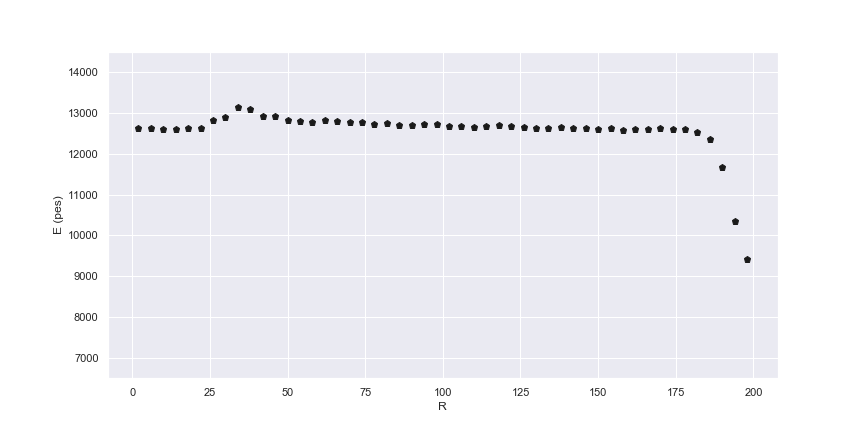
\includegraphics[width=0.7\textwidth]{img/r\runNumber x2rg_local_190819/RProfile.png}
    \caption{R profile shows that fiducial volume must be $R < 180$mm.}
  \end{center}
\end{figure}
\end{frame}


\begin{frame}
\frametitle{Profiles after $R < 180$mm}
\begin{figure}
  \begin{center}
      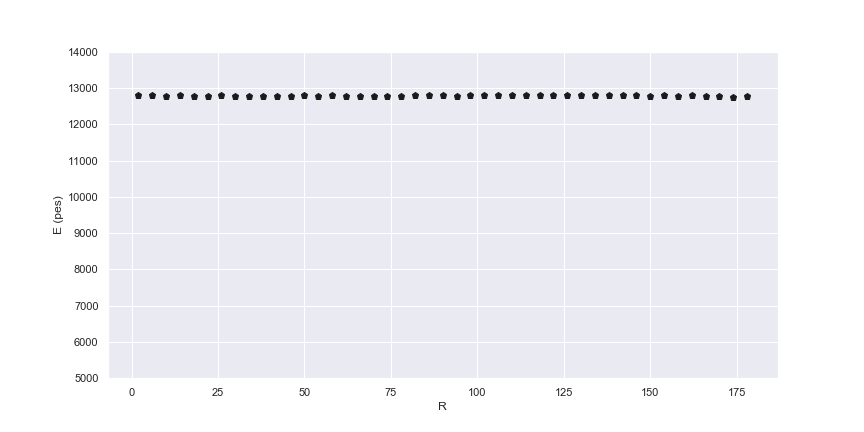
\includegraphics[width=0.4\textwidth]{img/r\runNumber x2rg_local_190819/RProfileC.png}
      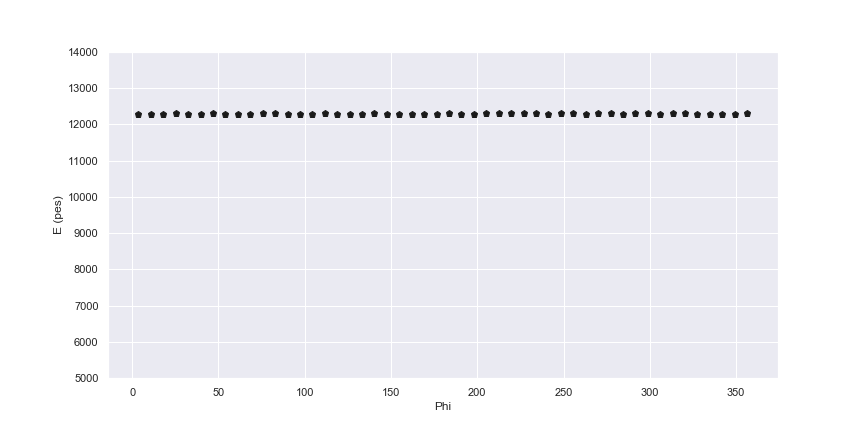
\includegraphics[width=0.4\textwidth]{img/r\runNumber x2rg_local_190819/PhiProfile.png} \\
      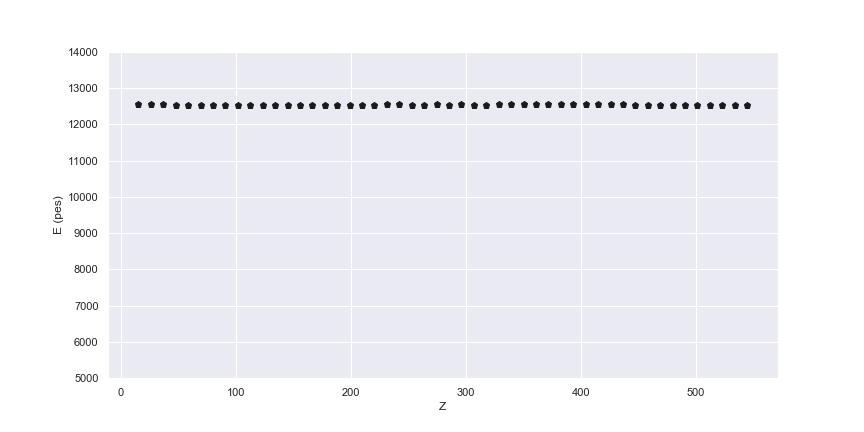
\includegraphics[width=0.4\textwidth]{img/r\runNumber x2rg_local_190819/ZProfile.png}
      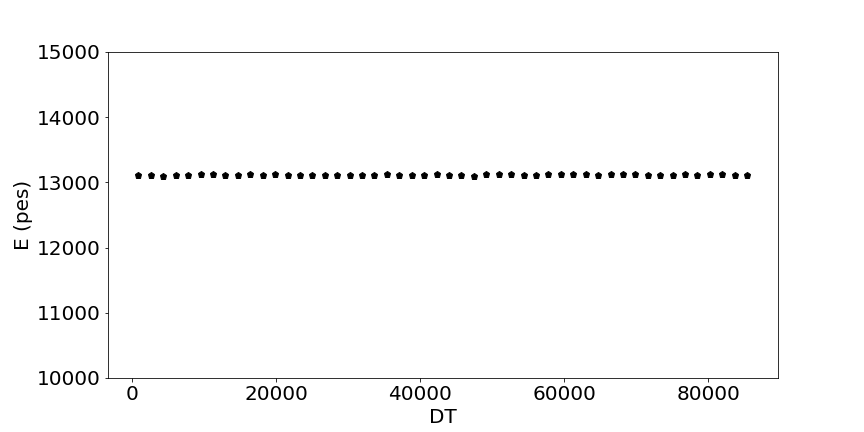
\includegraphics[width=0.4\textwidth]{img/r\runNumber x2rg_local_190819/TProfile.png}
    \caption{Profiles showing correction is robust.}
  \end{center}
\end{figure}
\end{frame}

\begin{frame}
\frametitle{Resolution fits as a function of R and Z}
\begin{figure}
  \begin{center}
      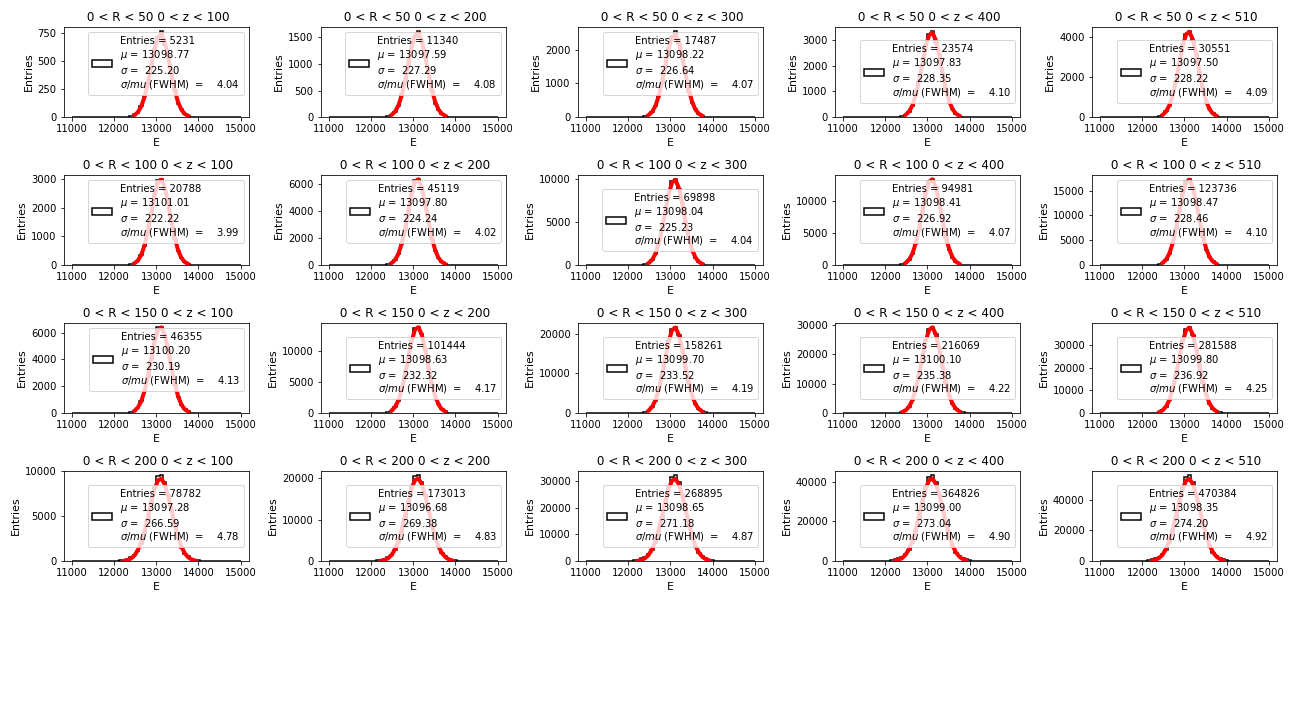
\includegraphics[width=0.8\textwidth]{img/r\runNumber x2rg_local_190819/ResoFit.png}
    \caption{Resolution fits.}
  \end{center}
\end{figure}
\end{frame}

\begin{frame}
\frametitle{Resolution as a function of R and Z}
\begin{figure}
  \begin{center}
      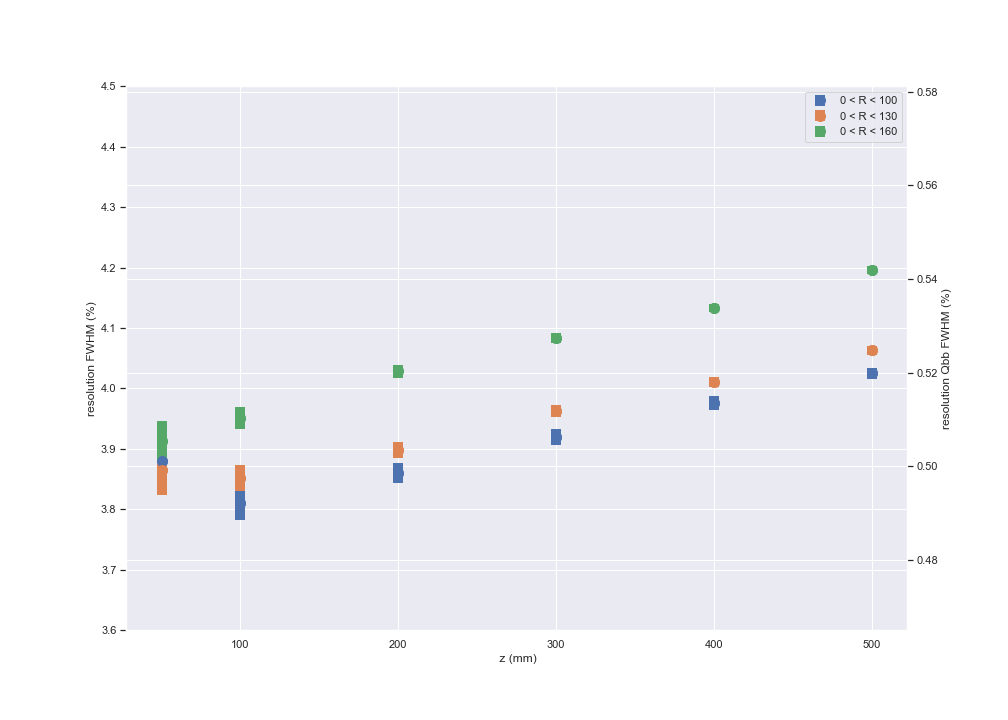
\includegraphics[width=0.8\textwidth]{img/r\runNumber x2rg_local_190819/ResoVsZR.png}
    \caption{Resolution fits.}
  \end{center}
\end{figure}
\end{frame}

\begin{frame}
\frametitle{Efficiency over time}
\begin{figure}
  \begin{center}
      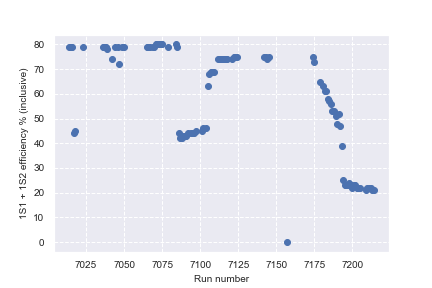
\includegraphics[width=0.8\textwidth]{img/r\runNumber x2rg_local_190819/EffVsTime.png}
    \caption{Efficiency tracking over time.}
  \end{center}
\end{figure}
\end{frame}

\begin{frame}
\frametitle{Response over time}
\begin{figure}
  \begin{center}
      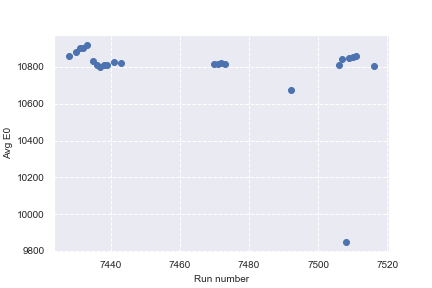
\includegraphics[width=0.8\textwidth]{img/r\runNumber x2rg_local_190819/E0VsTime.png}
    \caption{Response tracking over time.}
  \end{center}
\end{figure}
\end{frame}

\begin{frame}
\frametitle{Lifetime over time}
\begin{figure}
  \begin{center}
      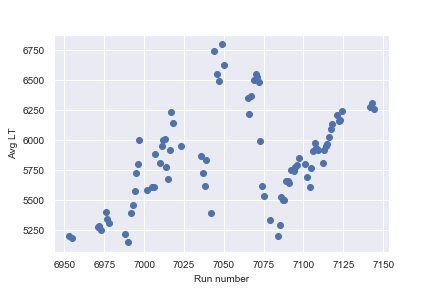
\includegraphics[width=0.8\textwidth]{img/r\runNumber x2rg_local_190819/LTVsTime.png}
    \caption{Lifetime tracking over time.}
  \end{center}
\end{figure}
\end{frame}

\begin{frame}
\frametitle{Resolution over time}
\begin{figure}
  \begin{center}
      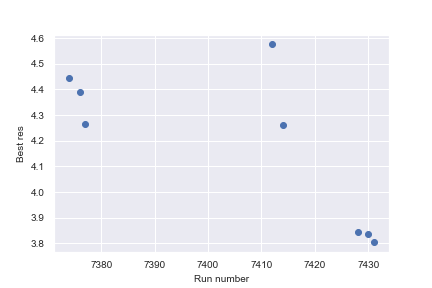
\includegraphics[width=0.8\textwidth]{img/r\runNumber x2rg_local_190819/ResVsTime.png}
    \caption{Resolution tracking over time.}
  \end{center}
\end{figure}
\end{frame}
